\documentclass{article}

\textwidth=6.5in
\textheight=8.5in
\voffset=-54pt
\oddsidemargin=0in
\evensidemargin=0in
\setlength{\parskip}{8pt}
\setlength{\parindent}{0pt}

\usepackage{amsmath, amssymb}
\usepackage{ifthen}

\usepackage[inline]{enumitem}
\setlist{topsep=0pt, parsep=8pt}

\usepackage[rgb,table]{xcolor}\convertcolorsUfalse
\usepackage{graphicx}

% change hyperref options
\PassOptionsToPackage{hyphens}{url}
\usepackage[bookmarks,colorlinks,linkcolor=black,citecolor=blue,pdfstartview=FitH,urlcolor=blue]{hyperref}
\hypersetup{pdfpagemode=UseNone}
\usepackage{bookmark}

\usepackage{graphicx}
\usepackage{multicol}
\usepackage{framed}
\usepackage{array}

\usepackage{icomma}

\usepackage{marginnote}
\usepackage[colorinlistoftodos]{todonotes}
\renewcommand{\marginpar}{\marginnote}

\usepackage{soul}

\usepackage{pgfplots}
\pgfplotsset{compat=1.18}  
\pgfplotscreateplotcyclelist{mycolor}{black, blue, red, green!70!black, magenta, purple, cyan, orange }  
\pgfplotsset{
  disabledatascaling,
  cycle list=tikzcolor, 
  axis lines=middle,
  every axis plot/.style={no marks, thick},
  every axis/.style={
    enlarge x limits=false,
    enlarge y limits=auto,
    xlabel style={at={(current axis.right of origin)},anchor=west},
    ylabel style={at={(current axis.above origin)},anchor=south},
    % extra x and y ticks for asymptotes
    extra x tick style={grid=major, grid style={dashed,black}},
    extra y tick style={grid=major, grid style={dashed,black}},
    /pgf/number format/1000 sep={},
  },    
  tick label style = {font=\footnotesize, fill=\currentbgcolor, inner sep=0pt},    
  xticklabel shift=1pt,    
  scaled ticks=false,
  scaled y ticks=false,
  unbounded coords=jump,
  samples=101,
  minor tick length=0,
  scatter/classes={
    open={mark=*,draw=black,fill=white, mark size=2, thin},
    closed={mark=*,draw=black,fill=black, mark size=2, thin}
  },
  width=3in,
}
\pgfplotsset{open/.style={only marks, mark=*, fill=white, thin, mark size=2}}
\pgfplotsset{closed/.style={only marks, mark=*, draw=black, fill=black,
    thin, mark size=2}}
\pgfplotsset{labeled/.style={nodes near coords, only marks, mark=*, draw=black, fill=black, thin, mark size=2, point meta=explicit symbolic}}

\usepackage{tikz}
\usetikzlibrary{
  matrix,%
  % enables the snake paths
  decorations.pathmorphing,%
  % enables bigger arrows
  decorations.markings,%
  decorations.pathreplacing,%
  decorations.text,%
  calc,%
  patterns,%
  shapes.geometric,%
  arrows,
  decorations.shapes,
  positioning,
  plotmarks,
  intersections
}
\tikzset{>=latex} % sets default arrow type in tikz
\tikzset{font=\normalsize}
\tikzset{mark size=1.5pt, mark options=thin}
\tikzset{pin distance=4pt,
  every pin edge/.style={<-, thin, shorten <= -2pt}}

\interfootnotelinepenalty=10000
\renewcommand{\thefootnote}{(\arabic{footnote})}

\usepackage{multirow, bigdelim}

% change to \usepackage[sols]{handout} to see solutions
\usepackage[]{handout}

\newcommand\iscurrentenumi[1]{%
  \ifthenelse{\equal{#1}{\theenumi}}{}{#1}}
\setenumerate[1]{ref=\#\arabic*}
\setenumerate[2]{ref=\protect\iscurrentenumi{\theenumi}(\alph*)}
\newcommand\enumiiprefix[2]{%
  \ifthenelse{{\equal{#1}{\theenumi}}\AND{\equal{#2}{(\alph{enumii})}}}{}{}%
  \ifthenelse{{\equal{#1}{\theenumi}}\AND{\NOT{\equal{#2}{(\alph{enumii})}}}}{#2}{}%
  \ifthenelse{\equal{#1}{\theenumi}}{}{#1#2}%
}
\setenumerate[3]{ref=\protect\enumiiprefix{\theenumi}{(\alph{enumii})}\roman*}

\newlength{\tipmargin}
\makeatletter

% underline links               
\let\@href=\href
\renewcommand{\href}[2]{\@href{#1}{\ul{#2}}}

\renewenvironment{framed}{
  \setlength{\tipmargin}{\textwidth-\linewidth}
  \advance\@totalleftmargin-\tipmargin
  \def\FrameCommand{\hspace{\tipmargin}\fbox}%
  \advance\linewidth\tipmargin
  \MakeFramed {\advance\hsize-\width \FrameRestore}%
}
{\endMakeFramed}

\makeatother

\definecolor{purple}{rgb}{0.5,0,1.0}

\usepackage{fancyhdr}
\lhead{\textcolor{white}{This content is protected and may not be shared, uploaded, or distributed.}}
\rhead{}
\rfoot{\vspace*{\fill}\footnotesize\textcopyright{} \emph{Harvard Math Ma}}
\renewcommand{\headrulewidth}{0pt}
\pagestyle{fancy}
\begin{document}

\htitle{Linear and Piecewise Linear Functions}

\begin{problemonly}
  \begin{framed}

You should be able to:
    \begin{itemize}[topsep=0pt,partopsep=0pt,parsep=8pt,itemsep=0pt] 
    \item Write the equation of a line given 2 points or 1 point and the
      slope, and decide whether slope-intercept form ($y = mx + b$) or
      point-slope form is more useful. 

    \item Use linear and piecewise linear equations to model various
      phenomena.

    \item Interpret the slope in linear and piecewise linear functions, 
      and graph the ``slope function'' $f'(x)$ of a piecewise linear
      function $f(x)$.  

    \end{itemize}
  \end{framed}
\end{problemonly}

\begin{enumerate}
\item  Economists use demand curves to express the relationship between the price of an item and the number of items customers want to buy (the ``demand''). Below is the demand curve for a certain good. $p$ is the price per item measured in dollars, and $q$ is the quantity of the good demanded (in other words, the number of items customers want to buy). 

  \begin{enumerate}
  \item

    \note{I'll have students try this; I expect many will try slope-intercept form. We'll talk about point-slope form and which seems easier.}

    \begin{problem}[0.75in]
      Based on the graph, express the demand $q$ as a function of the price $p$.\\
%ADDITIONAL NEED: Label axes, include units
      \begin{tikzpicture}
        \begin{axis}[xlabel=$p$, ylabel=$q$, xmin=0, ymin=0, xtick=\empty, ytick=\empty, width=2in, height=1.5in, clip=false, enlarge x limits=auto]
          \addplot+[domain=150:1000] {-4*(x-700)+2400}; %
          \addplot+[closed] coordinates {(450, 3400)} node[anchor=south west, inner sep=1pt]{$(450, 3400)$}; % 
          \addplot+[closed] coordinates {(750, 2200)} node[anchor=south west, inner sep=1pt]{$(750, 2200)$}; % 
        \end{axis}
      \end{tikzpicture}
    \end{problem}

    \begin{solution}
      We need the equation of a line, so we need a
      point and a slope. To find the slope, we use the two points we
      know and find the slope between them:
      $$\frac{2200 - 3400}{750 - 450} = -4$$
      So we get the following line:
      $$y - 2200 = -4(x-750)$$
      This means that $q$ as a function of $p$ is
      \[q(p) = -4(p-750)+2200\]
    \end{solution}

  \item
    \begin{problem}[\stretch{0.5}]
      In words, explain the meaning of the slope of the line.
    \end{problem}

    \begin{solution}
      The slope means that for every 1 dollar increase in
      price per item, the quantity of the good demanded decreases by 4
      units. 
    \end{solution}

  \item

    \note{Although we could write the line in point-slope form using either point, it's much easier to answer this question if we use the point (750, 2200). So, we see that sometimes we pick which equation to write for a line based on how we're going to use the line. (I won't mention this to students now, but this will be important when we approximate using secant lines or tangent lines.)}

    \begin{problem}[\vfill\newpage]
      If the item is priced at \$725, how many items will customers want to buy?
    \end{problem}

    \begin{solution}
      Based on our function, $q(725) = -4(725-750)+2200 = 2300$, so when the price per item
      is \$725, the quantity demanded will be 2300 units.
    \end{solution}

  \end{enumerate}

\item  Find an equation for each of the following lines.
  \begin{enumerate}

  \item
    \begin{problem}[\vfill]
      The line with slope $- \frac{1}{5}$ passing through the point $(23, 71)$. 
    \end{problem}

    \begin{solution}
      Using point-slope form, the equation is
      $\boxed{y - 71 = - \frac{1}{5} (x - 23)}$.

      Using slope-intercept form, the equation is
      $y = - \frac{1}{5} x + b$, and we can plug in the point $(23, 71)$
      to solve for $b$: $71 = -\frac{23}{5} + b$, so $b = \frac{378}{5}$, 
      and $\boxed{y = - \frac{1}{5} x + \frac{378}{5}}$. 
    \end{solution}

  \item
    \begin{problem}[\vfill]
      The line passing through the points $(0, p)$ and $(q, 0)$.
    \end{problem}

    \begin{solution}
      The slope is $\frac{0 - p}{q - 0} = - \frac{p}{q}$, 
      so the equation in point-slope form is
      $\boxed{y - p = - \frac{p}{q} x}$. 

      We can also write the equation in standard form:
      $\boxed{\frac{x}{q}+\frac{y}{p}=1}$.
    \end{solution}

  \end{enumerate}

\item 

  \note{This is just so that we have an explicit example of the open
    dot / closed dot convention in graphs and to remember how to write
    a piecewise formula.}

  In June 2023, the cost to send a letter through the \href{https://pe.usps.com/text/dmm300/Notice123.htm\#_c037}{US Postal Service} was:

  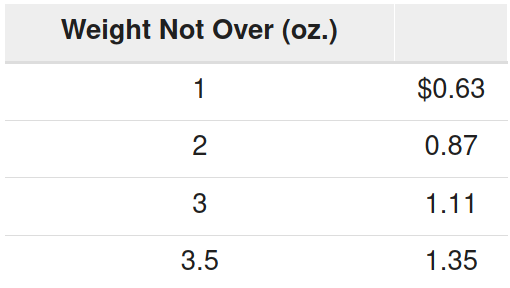
\includegraphics[width=2in]{images/usps.png}

  Let $C(w)$ be the cost to mail a letter weighing $w$ ounces.

  \begin{enumerate}
  \item
    \begin{problem}[\stretch{1.75}]
      Sketch the graph of $C(w)$. What is its domain? 
    \end{problem}

    \begin{solution}
        The domain is $(0, 3.5]$.
%ADDITIONAL NEED: label axes, include units
        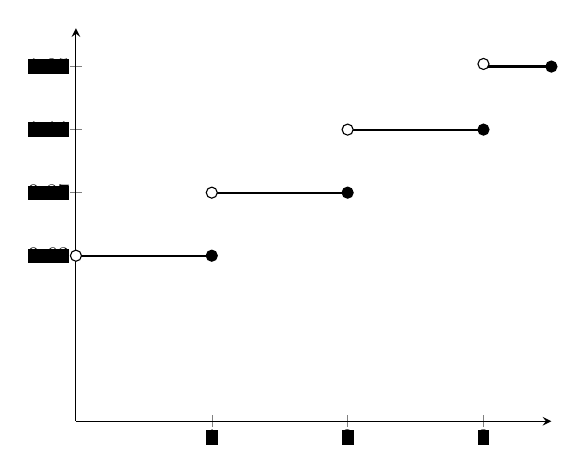
\begin{tikzpicture}
          \begin{axis}[ymin=0, ytick={0.63,0.87,1.11,1.35}]
            \addplot[domain=0:1]{0.63};
            \addplot[domain=1:2]{0.87};
            \addplot[domain=2:3]{1.11};
            \addplot[domain=3:3.5]{1.35};
            \addplot[open] coordinates {(0, 0.63) (1, 0.87) (2, 1.11) (3, 1.36)};
            \addplot[closed] coordinates {(1, 0.63) (2, 0.87) (3, 1.11) (3.5, 1.35)};
          \end{axis}
        \end{tikzpicture}
    \end{solution}

  \item
    \begin{problem}[0.15in]
      Is $C(w)$ continuous on its domain? 
    \end{problem}

    \begin{solution}
      No, the function is not continuous on its domain. We cannot draw the graph without
      picking up our pencil.
    \end{solution}

  \item
    \begin{problem}[\vfill\newpage]
      Write a formula for $C(w)$. 
    \end{problem}

    \begin{solution}
      We can write a piecewise formula.
      \[C(w)=
      \begin{cases}
        0.63 &\text{when } 0 < w \leq 1 \\
        0.87 &\text{when } 1 < w \leq 2 \\
        1.11 &\text{when } 2 < w \leq 3 \\
        1.35 &\text{when } 3 < w \leq 3.5
      \end{cases}
      \]
    \end{solution}

  \end{enumerate}

  \item 

  \note{This is an introduction to the slope function, through a two-piece piecewise example. Given our work using point-slope, this is a good opportunity for students to try to come up with the piecewise formula on their own and check whether they are on the right track, using the graph or computing the wages at various hours. Highlight the flexibility of how the graph can come together from the written description without depending on the overly technical algebraic formula.}

  Molly has just started a part time job that pays \$10 per hour for the first 6 hours that she works each week, and \$12 per hour for each hour after that. Molly is allowed to work up to 15 hours per week. Let $P(t)$ be Molly's income in a week if she works $t$ hours. 

  \begin{enumerate}

  \item
    \begin{problem}[\vfill]
      Find a formula for $P(t)$.
    \end{problem}

    \begin{solution}
      \[
        P(t)=
        \begin{cases}
          10t & 0 \leq x \leq 6\\
          12(t-6)+60& 6< x \leq 15  
        \end{cases}
      \]For the first 6 hours, she earns \$10 per hour, so the equation is simply $P(t) = 10t$. After that, she earns \$12 per hour, after earning \$60 from the first 6 hours, so we get $P(t) = 12(t-6) + 60$, until she's worked 15 hours that week, at which point, she has made:
      $$P(15) = 12(15-6) + 60 = 168$$
      dollars.
    \end{solution}

  \item
    \begin{problem}[\vfill]
      Sketch the graph of $P(t)$.
    \end{problem}

    \begin{solution}  The function is piecewise linear
      since on different parts of the domain the graph is a line with
      different slopes. In the picture below it is hard to tell. This is
      because a slope of 12 is visually not so different from a slope of
      10. \\
%ADDITIONAL NEED: Label axes, include units
      \begin{tikzpicture}
        \begin{axis}[axis lines=left, xmax=15.5,xtick={6,15}, ytick={60,168}]
          \addplot[domain=0:6]{10*x};
          \addplot[domain=6:15]{12*(x-6)+60};
          \addplot[closed] coordinates {(0,0) (6,60) (15,168)};
        \end{axis}
      \end{tikzpicture}

    \end{solution} 

  \item
    \begin{problem}[\vfill]
      Graph the ``slope function'' $P'(t)$. 
    \end{problem}

    \begin{solution}
      $P'(t)$ for the first 6 hours, 
      $0 < t < 6$, is given by the slope, \$10 per hour. Then, from
      $6<t<15$, $P'(t)$ is given by the slope, \$12 per hour. However, 
      at $t = 6$ and $t = 15$, $P'(t)$ is undefined.  

      \begin{tikzpicture} 
        \begin{axis}[ymin=0, xmax=17]
          \addplot+[domain=0:6] {10};
          \addplot+[domain=6:15] {12};
          \addplot[open] coordinates{(0, 10)(6, 10)(6, 12) (15, 12)};
        \end{axis}
      \end{tikzpicture}

      Notice the holes in the graph. These holes occur at
      points where the graph does not have a defined slope.  
    \end{solution}    

  \item
    \begin{problem}[0.5in]
      What is the practical meaning of $P'(t)$? Include units in your
      answer.
    \end{problem}

    \begin{solution}
      $P'(t)$ gives us the number of dollars Molly makes
      per hour if she's already worked $t$ hours.
    \end{solution}

  \end{enumerate}

\begin{problemonly}
    
\newpage
\end{problemonly}
\item  \label{thomas-wolfe}

  \note{This is a great problem to have students work on at the board. It's also a great opportunity to discuss problem solving strategies. For example:
    \begin{itemize}
    \item Computing concrete examples is really helpful. (What would Wolfe earn if he sold 2000 copies? 3001 copies? 4501 copies?) The process you use to calculate each example is easy to generalize to give you the formula for one piece of the graph. (And, more generally, doing concrete examples is just a great mathematical strategy.)

    \item Sketching the graph from the verbal description is much easier than trying to sketch it from the algebraic formula.

      More generally, being flexible about what information you use (verbal description, algebraic formula, graphical information) is valuable when solving problems.
    \end{itemize}
  }

  Instead of a straight royalty percentage on sales of his book, 
  \textit{The Story of a Novel}, the author Thomas Wolfe agreed to accept
  a sliding scale of 10\% on the first 3000 copies sold, 20\% on the next
  1500 copies, and 30\% on all copies after that. The book was priced at
  \$2.\footnote{The numbers in this problem have been modified for
    computational ease.}

  \begin{enumerate}
  \item \label{thomas-wolfe-formula}

    \begin{problem}[\vfill]
      Write a function $R(x)$ that gives Wolfe's royalties as a function
      of $ x$, the number of books sold.
    \end{problem}

    \begin{solution} 
      The amount of money that Wolfe collects depends on the number of books sold. Marginal income is the amount of income generated from selling one more book. In this situation the marginal income changes. To tackle the sliding scale we will make use of a piecewise function. 
      \[
        R(x)=
        \begin{cases}
          0.2 x & \text{ if } 0 \leq x \leq 3000, \\
          0.4 (x-3000) +600  & \text{ if } 3000 < x \leq 4500, \\
          0.6(x-4500) + 1200 & \text{ if } 4500 < x
        \end{cases}
      \]
      If you did not come up with this formula or an equivalent one, ask yourself what is the purpose of $(x-3000)$ and the $(x-4500)$? We are subtracting 3000 from $x$ because we are making $40$ cents on sales over $3000$ books. As always trying an \textcolor{blue}{ concrete example}  helps. To calculate $R(4500)$ we would make 20 cents on the first 3000 and we would make 40 cents on the next 1500 books. $$R(4500) = 0.4(1500)+0.2(3000)=1200$$

    \end{solution} 

  \item \label{thomas-wolfe-graph}
    \begin{problem}[\vfill]
      Graph $R(x)$.
    \end{problem}
%ADDITIONAL NEED: label axes include units

    \begin{solution} 
      \begin{center}
        \begin{tikzpicture}
          \begin{axis}[
          axis lines=left, 
          xlabel=\textit{books sold},
          ylabel = \textit{royalties earned in dollars},
          xtick={3000, 4500}, ytick={600, 1200}]
            \addplot+[domain=0:3000] {.20*x};
            \addplot+[domain=3000:4500] {.40*(x-3000) +600};
            \addplot+[domain=4500:6000] {.60(x-4500) +1200};
          \end{axis}
        \end{tikzpicture}
      \end{center}
    \end{solution} 

  \item
    \begin{problem}[\vfill\newpage]
      Do some sort of check of whether your answer to \ref{thomas-wolfe-formula} is sensible, as well as whether it agrees with your graph in \ref{thomas-wolfe-graph}. (How you decide to check is up to you; thinking of a good way to check is part of the challenge!)
    \end{problem}

    \begin{solution}
      One check we could perform on our formula for $R(x)$ is to test various inputs and check
      if we get the expected outputs.
    \end{solution}

  \item

    \note{This part is less important, so if we're running short on time, I'll have students skip this so they can look at the next 2 parts.}

    \begin{problem}[\vfill]
      Solve $R(x) = 900$. What does this equation mean?
    \end{problem}

    \begin{solution} 
      We need to solve the equation $R(x) = 900$. From our previous work we know that if we sell 3000 books we have made $\$600$ and if we sell 4500 books we have made $\$1200$. This means that algebraic rule we should be using is the rule for selling between 3000 and 4500 books.  
      $$0.4(x-3000) +600 =900$$ 
      $$0.4x -1200+600=900$$
      $$0.4x-600=900$$
      $$0.4x=1500$$
      $$x =3750$$
      The solution means that he needs to sell 3750 books to make $\$900$. 
    \end{solution} 

  \item

    \note{Make sure to talk about the fact that $R'$ is undefined where the slope changes, and have students figure out how to depict that in their graphs.

      Technically, $R'$ is also undefined at 0, but we won't be picky about this. }

    \begin{problem}[\vfill]
      Graph the ``slope function'' $R'(x)$, which gives the slope at every
      point on the graph of $R$. 
    \end{problem}

    \begin{solution} 
    We know the slopes of the three linear pieces. At the $x$-values
    where different pieces meet, there is no single slope, so we leave
    $R'(x)$ undefined for those points.
% ADDITIONAL NEED: Label axes and include units
      \begin{tikzpicture} 
        \begin{axis}[ymin=0,xtick={3000,4500}]
          \addplot+[domain=0:3000] {.2};
          \addplot+[domain=3000:4500] {.4};
          \addplot+[domain=4500:6000] {.6};
          \addplot[open] coordinates{(0, .2) (3000, .2)(3000, .4)(4500, .4)(4500, .6)};
        \end{axis}
      \end{tikzpicture} 
    \end{solution} 

  \item

    \note{It's good to be explicit about how $x$ is involved here, so something like ``the royalties Wolfe earns for selling an additional book if he's already sold $x$ books'' (and emphasize the units are dollars per book, not dollars). Of course, we'll eventually see that $R'(x)$ is an instantaneous rate of change, so it isn't really about selling 1 more book, but this is a good enough understanding for now.}

    \begin{problem}[\nstretch{0.25}]
      What's the practical meaning of $R'(x)$? Include units in your answer.
    \end{problem}

    \begin{solution} 
      $R'(x)$ gives the royalties earns (in dollars per book) if he's already sold $x$ books.
    \end{solution} 

  \end{enumerate} 


\end{enumerate}
\end{document}
